\documentclass{beamer}

\usepackage{graphicx}
\usepackage{hyperref}
\usepackage[latin1]{inputenc}
\usepackage[T1]{fontenc}
\usepackage[english]{babel}
\usepackage{listings}
\usepackage{xcolor,mathrsfs,url}
\usepackage{amssymb}
\usepackage{amsmath}
\usepackage{ifthen}

% The command to define a subsection is '\subsec{}' and NOT '\subsection'.
% This code generates the bar. Don't edit.
\newcommand{\midbarnew}{}
\newcommand{\subsec}[1]
{
  \ifthenelse{\equal{#1}{}}
  {\renewcommand{\midbarnew}{} \subsection{}}
  {\renewcommand{\midbarnew}{ $\mid$ } \subsection{#1}}
}

% change the pictures here, if necessary. logobig and logosmall are the internal names
% for the pictures: do not modify them, just change "hulogo" and "logo". Pictures must be 
% supplied as JPEG, PNG or PDF
%########################################

% \pgfdeclareimage[height=2cm]{logobig}{logo} % use hucase instead for the Humboldt-Case Logo
% \pgfdeclareimage[height=1cm]{logosmall}{logo}

% use this number to modify the scaling of the headline on titlepage

\title{Trade Policy: Part One}
\author{Instructor: David Jinkins\thanks{I wish to acknowledge Battista Severgnini for providing last year's slides to me. His generosity saved me much time, and these slides are partially based on his. Any errors are of course my own.}}
\date{Date: Sept. 23, 2014}

%Start of the document
\begin{document}

\frame{\titlepage}

\begin{frame}
    \begin{itemize}
    \itemsep1pt\parskip0pt\parsep0pt
    \item
      Last time: Increasing Returns to Scale
      \begin{itemize}
            \item Krugman: External Economies 
            \begin{itemize}
                \item Larger industries have lower cost
                \item Drives industries to concentrate
                \item A reason for trade
            \end{itemize}
            \item Implications of external economies 
            \begin{itemize}
                \item Historical Accident
                \item Money on the table
                \item Infant industries
            \end{itemize}
            \item Melitz and Krugman: Internal Economies
            \begin{itemize}
                \item Larger firms have lower cost 
                \item Each firm a different product or variety
                \item Consumers like a mix
                \item Reason for trade: more (and cheaper) varieties
            \end{itemize}
        \end{itemize}
    \end{itemize}
\end{frame}

\frame{% how to print
\frametitle{Plan for Today}
Chapter 8:
\begin{itemize}
\item Review: Monopoly
\item Review: Monopolistic competition
\item New: Trade costs
\item New: Dumping
\item New: Multinationals
\end{itemize}
Chapter 9 : 
\begin{itemize}
\item Tariffs
\item Consumer \& Producer Surplus
\item Export Subsidies
\end{itemize}
Chapter 10 :
}

\begin{frame}{Review}
    \begin{itemize}
        \item Begin review
    \end{itemize}
\end{frame}

\frame[plain]{
\includegraphics[page=26,width=\textwidth]{scale_and_trade.pdf}}
\frame[plain]{
\includegraphics[page=27,width=\textwidth]{scale_and_trade.pdf}}
\frame[plain]{
\includegraphics[page=32,width=\textwidth]{scale_and_trade.pdf}}
\frame[plain]{
\includegraphics[page=33,width=\textwidth]{scale_and_trade.pdf}}
\frame[plain]{
\includegraphics[page=34,width=\textwidth]{scale_and_trade.pdf}}
\frame[plain]{
\includegraphics[page=35,width=\textwidth]{scale_and_trade.pdf}}
\frame[plain]{
\includegraphics[page=37,width=\textwidth]{scale_and_trade.pdf}}
\frame[plain]{
\includegraphics[page=38,width=\textwidth]{scale_and_trade.pdf}}
\frame[plain]{
\includegraphics[page=39,width=\textwidth]{scale_and_trade.pdf}}
\frame[plain]{
\includegraphics[page=40,width=\textwidth]{scale_and_trade.pdf}}
\frame[plain]{
\includegraphics[page=41,width=\textwidth]{scale_and_trade.pdf}}
\frame[plain]{
\includegraphics[page=43,width=\textwidth]{scale_and_trade.pdf}}
\frame[plain]{
\includegraphics[page=44,width=\textwidth]{scale_and_trade.pdf}}
\frame[plain]{
\includegraphics[page=46,width=\textwidth]{scale_and_trade.pdf}}
\frame[plain]{
\includegraphics[page=47,width=\textwidth]{scale_and_trade.pdf}}
\frame[plain]{
\includegraphics[page=48,width=\textwidth]{scale_and_trade.pdf}}
\frame[plain]{
\includegraphics[page=51,width=\textwidth]{scale_and_trade.pdf}}
\frame[plain]{
\includegraphics[page=52,width=\textwidth]{scale_and_trade.pdf}}
\frame[plain]{
\includegraphics[page=53,width=\textwidth]{scale_and_trade.pdf}}
\frame[plain]{
\includegraphics[page=54,width=\textwidth]{scale_and_trade.pdf}}
\frame[plain]{
\includegraphics[page=57,width=\textwidth]{scale_and_trade.pdf}}
\frame[plain]{
\includegraphics[page=58,width=\textwidth]{scale_and_trade.pdf}}
\frame[plain]{
\includegraphics[page=59,width=\textwidth]{scale_and_trade.pdf}}
\frame[plain]{
\includegraphics[page=60,width=\textwidth]{scale_and_trade.pdf}}
\frame[plain]{
\includegraphics[page=63,width=\textwidth]{scale_and_trade.pdf}}
\frame[plain]{
\includegraphics[page=67,width=\textwidth]{scale_and_trade.pdf}}
\frame[plain]{
\includegraphics[page=68,width=\textwidth]{scale_and_trade.pdf}}
\frame[plain]{
\includegraphics[page=70,width=\textwidth]{scale_and_trade.pdf}}
\frame[plain]{
\includegraphics[page=72,width=\textwidth]{scale_and_trade.pdf}}

\begin{frame}
    \begin{itemize}
        \item End review!
    \end{itemize}
\end{frame}

\begin{frame}{Trade Costs and Extensive Margin} 
    \begin{itemize}
        \item Suppose there is some cost to trade 
        \item Equivalent to increasing marginal cost of production
        \item Recall firms with high marginal cost don't enter domestic market 
        \item Even fewer firms will enter the export market
        \item \emph{Extensive margin}: Number of firms exporting
        \item \emph{Intensive margin}: How much each firms export
        \item Trade costs reduce both
    \end{itemize}
\end{frame}

\begin{frame}{Extensive Margin is important} 
    \begin{itemize}
        \item Small share of firms export -- 18\% of American firms overall 
    \end{itemize}
    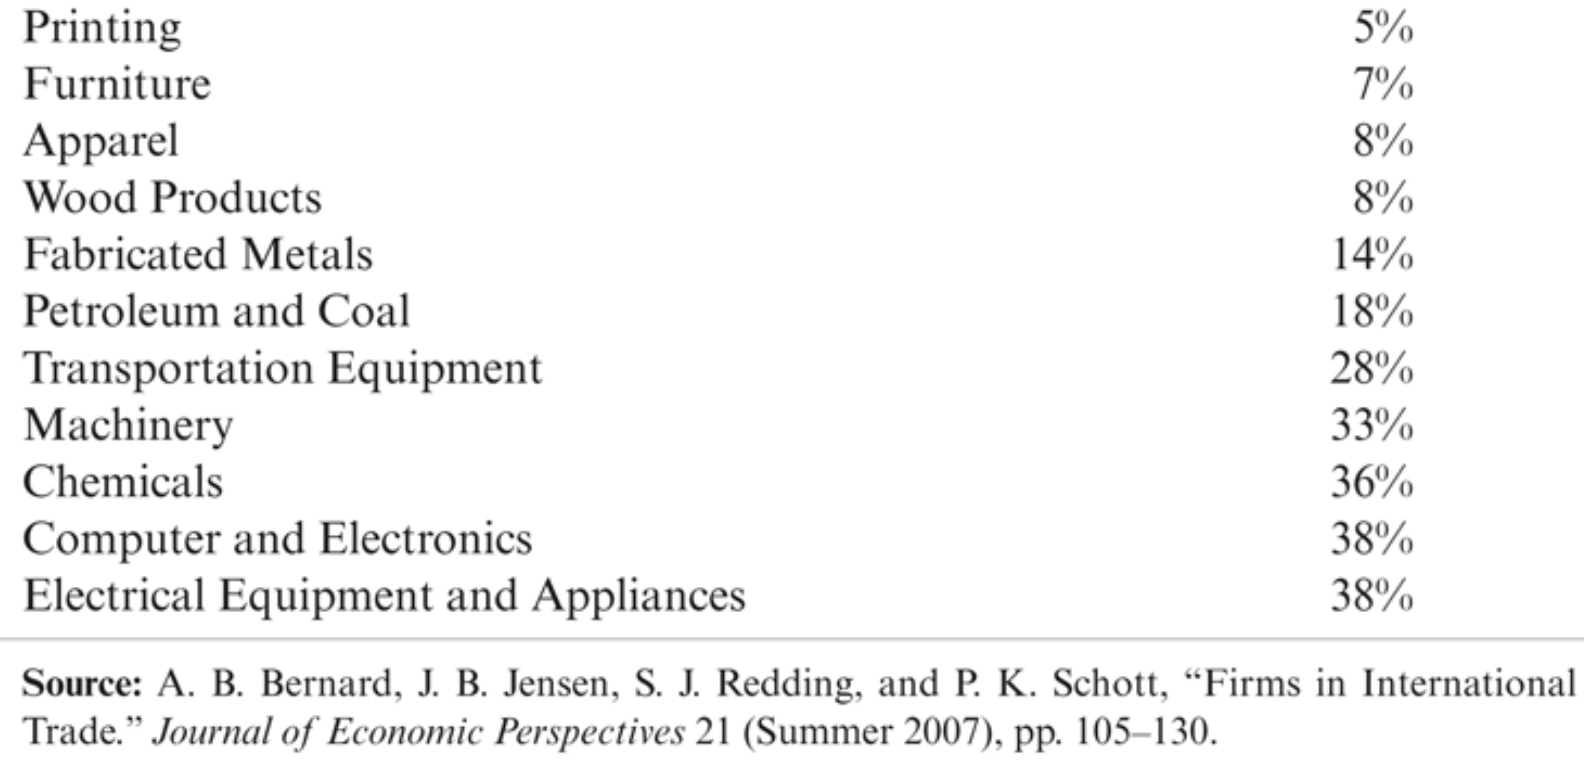
\includegraphics[scale=0.20]{bjrs_firms.png}
\end{frame}

\begin{frame}{Extensive Margin in a Picture} 
    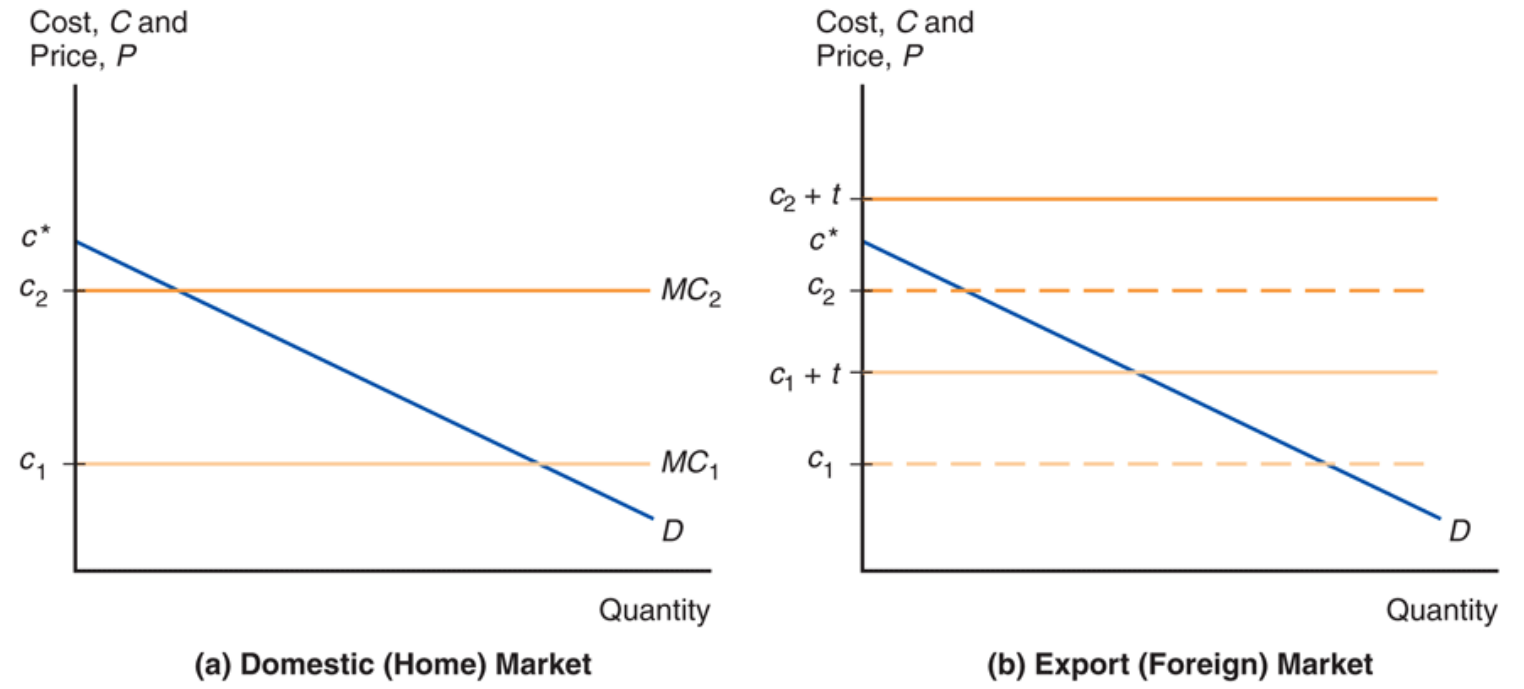
\includegraphics[scale=0.20]{trade_costs_firms.png}
\end{frame}

\begin{frame}{Predictions of Heterogenous Firms with Trade Cost}
    \begin{itemize}
        \item Subset of firms export
        \item Those that do are relatively productive
        \item Largely backed up by data:
        \begin{itemize}
            \item Exporters on average twice as large as importers (size vs. prod?)
            \item Produce on average 11\% more per worker
        \end{itemize}
    \end{itemize}
\end{frame}

\begin{frame}{Dumping}
    \begin{itemize}
        \item \emph{Dumping} is when a firm sells a product too cheaply abroad
        \begin{enumerate}
            \item Sometimes if foreign price below domestic price 
            \item Sometimes if foreign price below domestic price plus tariff
            \item Sometimes if foreign price is below cost of production
        \end{enumerate}
        \item Considered an unfair trade practice, WTO allows 'antidumping duty' or tariff
        \item Monopolistic competitive firms naturally do No. 2 (but not No. 1 or No. 3)
        \item Why?
        \item Textbook: This is just natural firm behavior 
        \item Me: Don't feel too bad -- these firms are still monopolists!
    \end{itemize}
\end{frame}

\begin{frame}{Pause}

    \begin{itemize}
        \item Trade costs: exporters on average more productive
        \item Dumping: Depending on definition, natural behavior
        \item Now: Foreign Direct Investment
        \item Note: Not directly related to increasing returns
        \item Included because firm behavior in trade
    \end{itemize}

\end{frame}

\begin{frame}{Foreign Direct Investment}

    \begin{itemize}
        \item Comes in two flavors
        \begin{enumerate}
            \item \emph{Vertical}: Do manufacturing where it is cheap
            \item \emph{Horizontal}: Produce close to final market
        \end{enumerate}
        \item Vertical example: iPhones made in China, designed in California
        \item Horizontal example: Japanese cars produced in the United States
    \end{itemize}

\end{frame}

\begin{frame}{Motives for FDI}
    \begin{itemize}
        \item Vertical FDI
        \begin{itemize}
            \item ex: Take advantage of lower labor costs abroad
            \item Capital can move: Factor price equalization all over again!
        \end{itemize}
        \item Horizontal FDI
        \begin{itemize}
            \item Proximity-Cost tradeoff
            \item Language developed by my professor, Steven Yeaple (along with Melitz)
            \item Low transport cost, export more
            \item High transport cost, build factor abroad
            \item Prediction consistent with data
        \end{itemize}
    \end{itemize}
\end{frame}

\begin{frame}{Outsourcing and Offshoring}
    \begin{itemize}
        \item In both flavors of FDI, keep transactions in the firm?
        \item Vertical
        \begin{itemize}
            \item Should you buy intermediates from foreign frim?
            \item Or build a factor abroad?
        \end{itemize}
        \item Horizontal
        \begin{itemize}
            \item Should you license technology to local producer?
            \item Or open a foreign factory yourself?
        \end{itemize}
        \item These are deep and difficult questions
        \item Depend on the theory of the firm
        \begin{itemize}
            \item Economics about the power of the market
            \item Each firm is a tiny communist country 
        \end{itemize}
    \end{itemize}
\end{frame}

\begin{frame}{Offshoring increasingly important}

    \begin{itemize}
        \item Intermediates are 40\% of manufactures trade (which are around 55\% of world trade)
        \item Intra-firm trade is 30\% of world trade
        \item Frontier of research, no definitive motive for internalization
    \end{itemize}

\end{frame}

\begin{frame}{Chapter 8: Summary}

    \begin{itemize}
        \item Monopolistic Competition
        \item Fixed cost give increasing return to scale
        \item Model for analyzing firms and trade (why?)
        \item Trade grows productive firms, shrinks unproductive firms
        \item Effect like productivity growth
        \item Frontier of research: FDI and internalization decisions
    \end{itemize}

\end{frame}

\frame{
\begin{center}
\textcolor{blue}{\textbf{Chapter 9: The Instruments of Trade Policy}}
\end{center}
}

\frame{
\frametitle{Chapter 9-12}
\begin{itemize}
\item First 8 chapters: 
    \begin{itemize}
        \item Why do countries trade?
        \item Is more trade generally good or bad?
        \item How does trade affect income distribution?
        \item How does trade affect firms?
    \end{itemize}
\item Chapters 9-12: 
    \begin{itemize}
        \item How does trade policy affect welfare?
        \item How is trade policy formed?
        \item When is trade policy justified?
        \item Open trade policy questions and the future
    \end{itemize}
\item Except for 9, these chapters are for the most part ``chatty''
\end{itemize}
}

\begin{frame}{Chapter 9}

    \begin{itemize}
        \item How do tariffs affect trade?
        \item How do tariffs affect welfare?
        \item How do other trade policy tools affect welfare?
    \end{itemize}

\end{frame}

\begin{frame}{Partial Equilibrium}

    \begin{itemize}
        \item Previous chapters (mostly) general equilibrium
        \begin{itemize}
            \item Begin with market structure, factor endowments, or available technology
            \item All prices determined in equilibrium (think relative price in our models)
            \item Equilibrium conditions like balance of trade, marginal cost equals marginal revenue, etc
            \item Income effects, substitution effects
        \end{itemize}
        \item Tariff analysis is partial equilibrium
        \begin{itemize}
            \item Only concerned with a single good, single price
            \item Strong assumption: Neither incomes nor other prices change
            \item Welfare only affected by consumption or sale of the single good
        \end{itemize}
    \end{itemize}

\end{frame}

\frame{
\frametitle{Tariffs}
Two types of tariffs:
\begin{enumerate}
\item \textbf{specific tariff:} fixed charge for each \textit{unit} of imported goods (e.g., 1 DKK per kg of cheese)
\begin{center}
$P=P^{*}+t$
\end{center}
\item \textbf{\textit{ad valorem} tariff:} fraction of the \textit{value} of imported goods (e.g., 25\% tariff on the value of imported cars) 
\begin{center}
$P=P^{*}\left(1+\tau\right)$
\end{center}
\end{enumerate}
\begin{itemize}
    \item Most discussion today: Specific tariff
    \item Most tariffs today: Ad valorem tariff
    \item Distinction will not change analysis much
\end{itemize}
}

\frame{
\frametitle{Tariffs in history}
\begin{itemize}
    \item Tariffs were \emph{the} source of government revenue for much of history
    \item Easy to put government agents at ports
    \item Same reason Turkey has extremely high petrol tax
    \item Because of tariffs, good international trade data is unusually detailed and old
\end{itemize}
}

\begin{frame}{19th century US tariffs}

    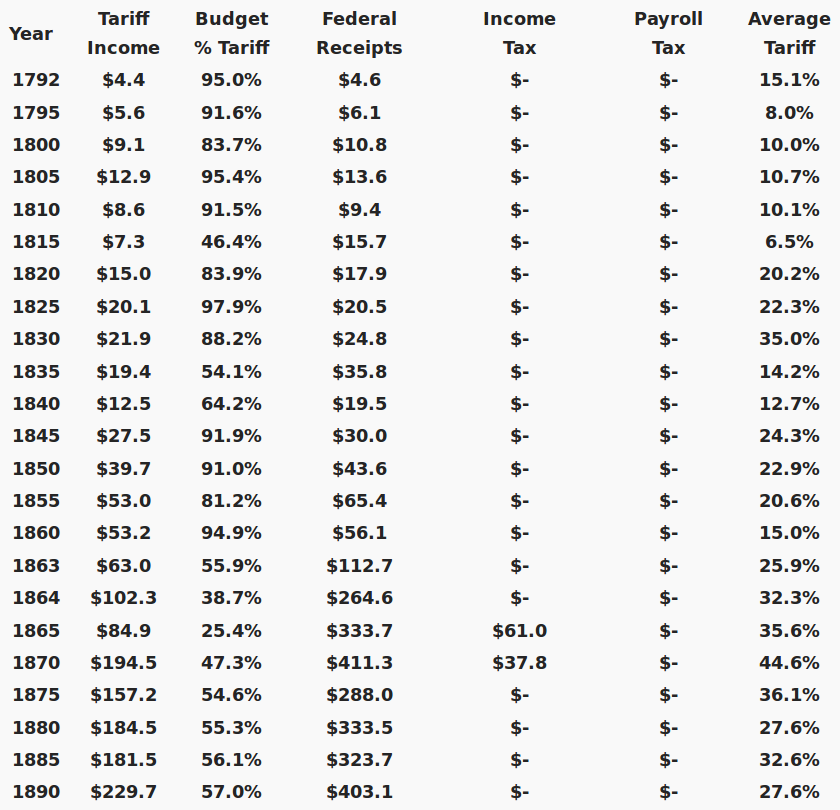
\includegraphics[scale=0.25]{US_tariffs_19th.png}

    {\tiny source: http://en.wikipedia.org/wiki/Tariffs\_in\_United\_States\_history}

\end{frame}

\begin{frame}{20th century US tariffs}

    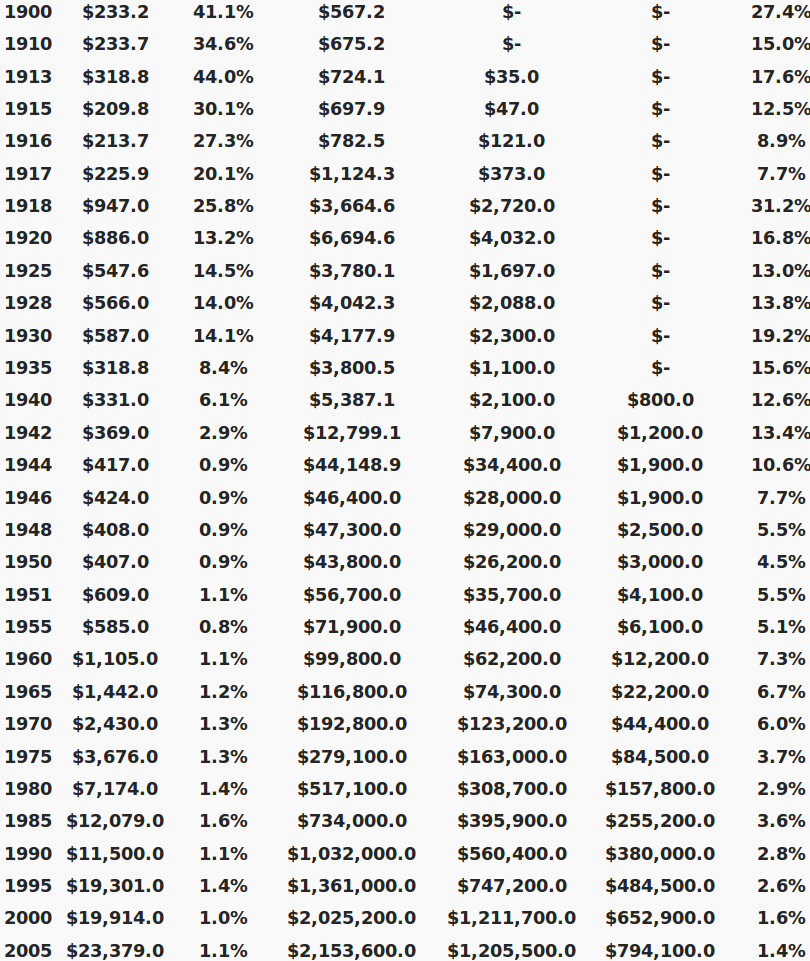
\includegraphics[scale=0.25]{US_tariffs_20th.png}

    {\tiny source: http://en.wikipedia.org/wiki/Tariffs\_in\_United\_States\_history}

\end{frame}

\frame{
\frametitle{Import Demand Curve}
\begin{itemize}
    \item Import demand curve 
    \begin{itemize}
        \item Y-axis price
        \item X-axis The difference between the quantity that domestic consumers demand and the quantity domestic producers supply
    \end{itemize}
\end{itemize}
}

\frame{
\frametitle{Export Supply Curve}
\begin{itemize}
    \item Export Supply Curve 
    \begin{itemize}
        \item Y-axis price
        \item X-axis The difference between the quantity that foreign produce supply and the quantity foreign supply
    \end{itemize}
\end{itemize}
}

\frame{
\frametitle{Import Demand Curve}
\begin{figure}
	\centering
		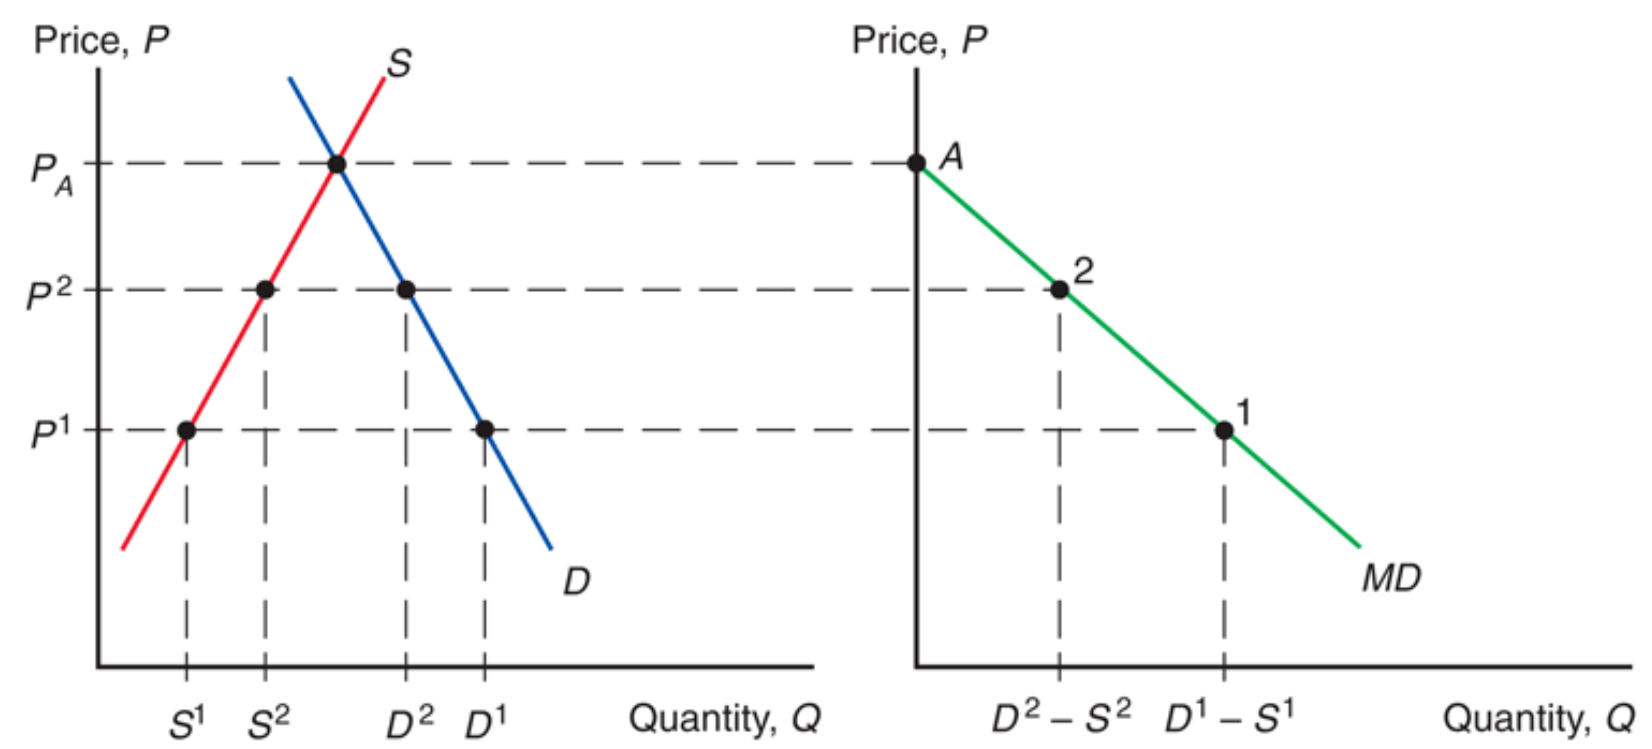
\includegraphics[width=0.80\textwidth]{import_demand.png}
\end{figure}
}

\frame{
\frametitle{Export Supply Curve}
\begin{figure}
	\centering
		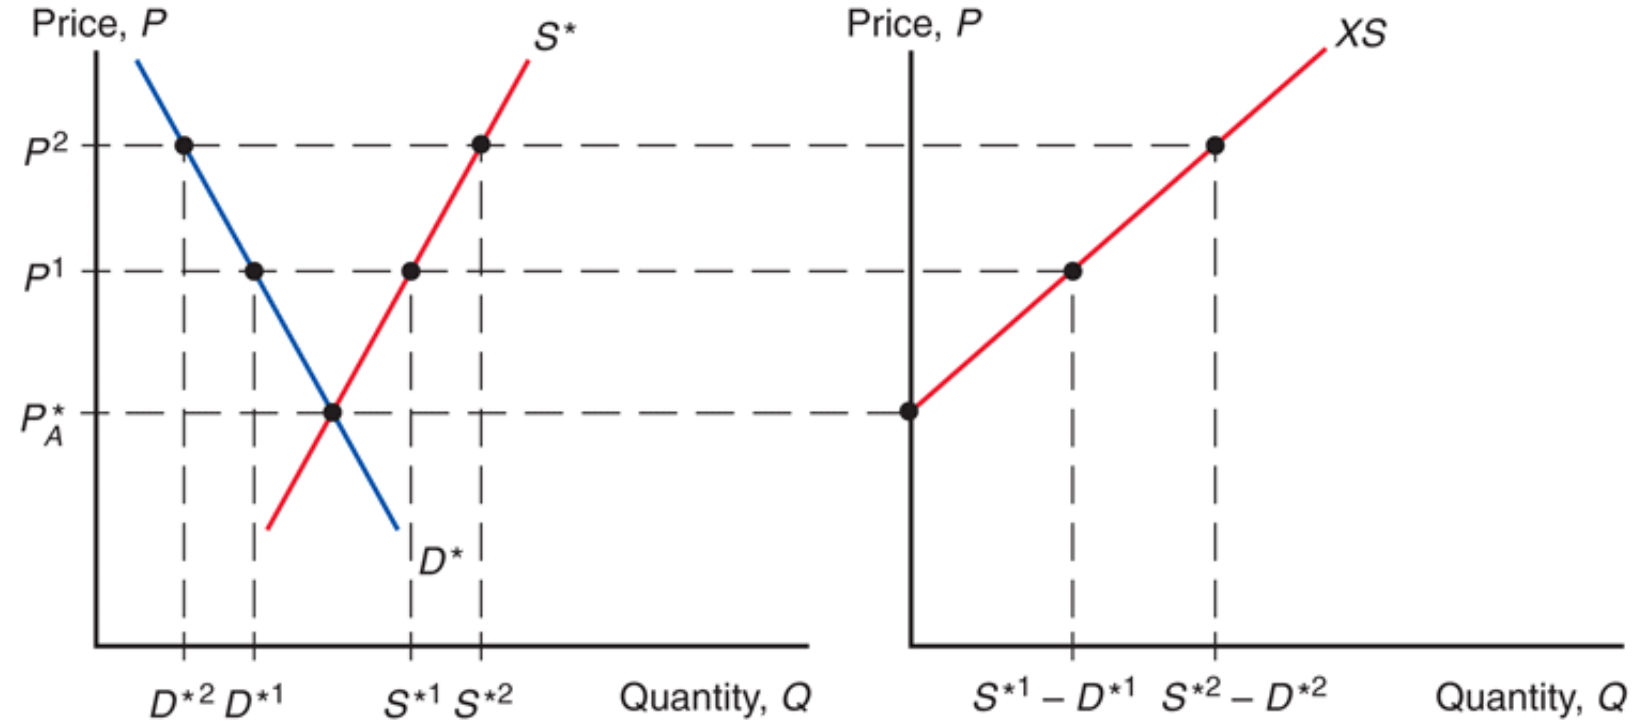
\includegraphics[width=0.80\textwidth]{export_supply.png}
\end{figure}
}

\frame{
\frametitle{World Market Equilibrium}
Combine XS and MD curves: equilibrium price and quantity at
the world market.
In equilibrium
\begin{itemize}
\item import demand = export supply
\item domestic demand - domestic supply =foreign supply - foreign demand ($D-S=S^{*}-D^{*}$)
\item world demand = world supply ($D+D^{*}=S^{*}-S$)
\end{itemize}
}

\frame{
\frametitle{World Equilibrium}
\begin{figure}
	\centering
		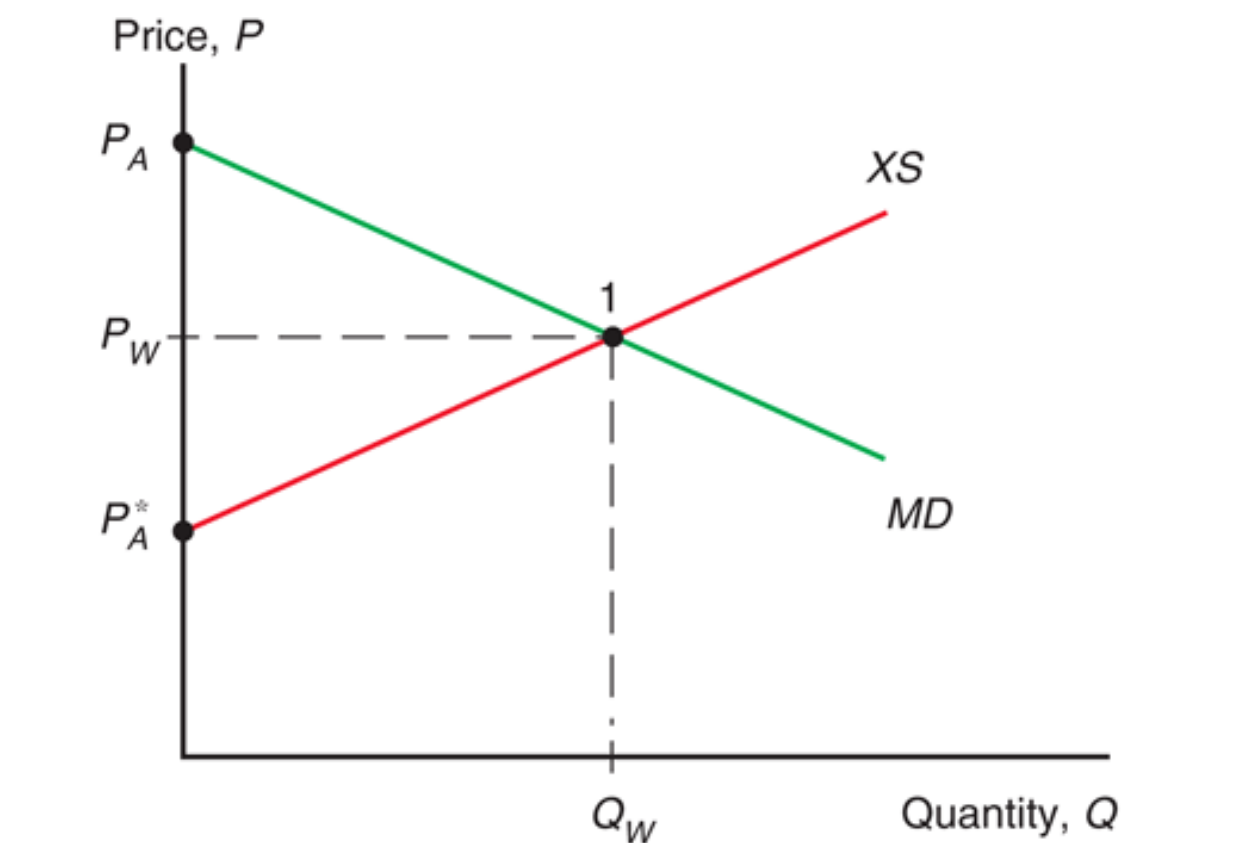
\includegraphics[width=0.80\textwidth]{world_equil.png}
\end{figure}
}

\frame{
\frametitle{The Effects of a Tariff}
\begin{itemize}
\item Sellers only sell abroad if the foreign price is greater than the domestic price plus the tariff. Why?
\item Sellers only sell domestically if the foreign price is less than than the domestic price plus the tariff. Why?
\item Equilibrium price difference is the tariff:
\begin{center}
$P_{T} - P^{*}_{T} = t $
\end{center}
\item Just after the tariff is set, there is excess demand at Home, and excess supply at Foreign
\item Price adjusts up at Home, and down in Foreign
\item Imports into Home and exports from Foreign are reduced
\item Price changes depend on shape of import demand and export supply
\end{itemize}
}
  
\frame{
\frametitle{Tariff and Price}
    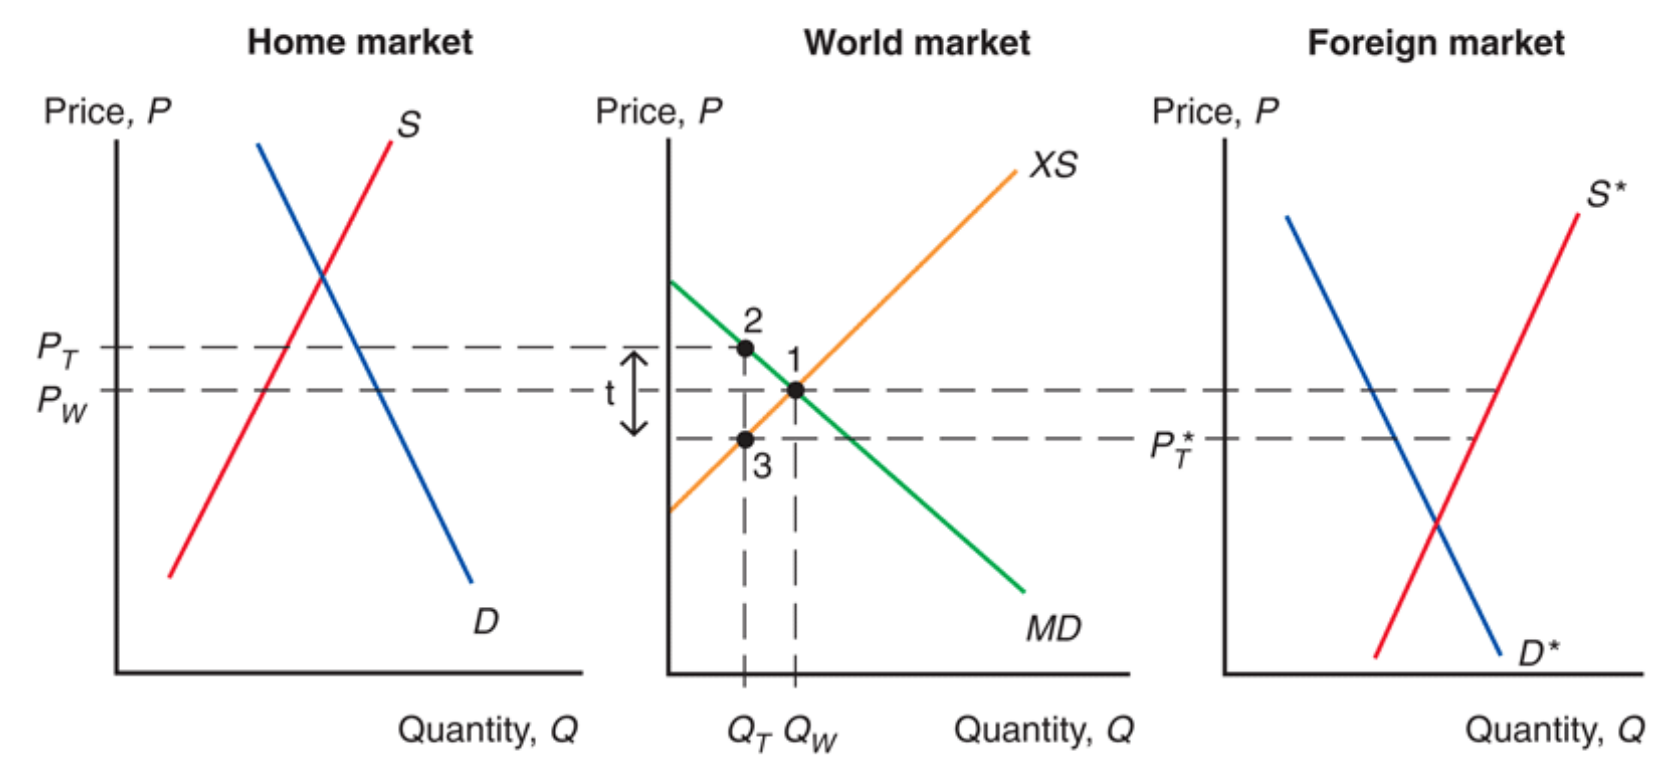
\includegraphics[width=0.80\textwidth]{tariff_prices.png}
}
  
\begin{frame}{Price determination}

    \begin{itemize}
        \item What would it mean if export supply were flatter?
        \begin{itemize}
            \item Elastic supply or demand cause prices to move less 
            \item If Home is only a minor destination, supply and demand in Foreign very elastic
            \item If Foreign drops price a small amount, a great deal more is demanded (relative to Home)
            \item If Foreign drops price a small amount, a great less is supplied  (relative to Home)
        \end{itemize}
        \item If foreign supply perfectly elastic, Home prices rise the same amount as the tariff
    \end{itemize}

\end{frame}
  
\frame{
\frametitle{Small Home,  Flat Export Supply}
\begin{figure}
	\centering
		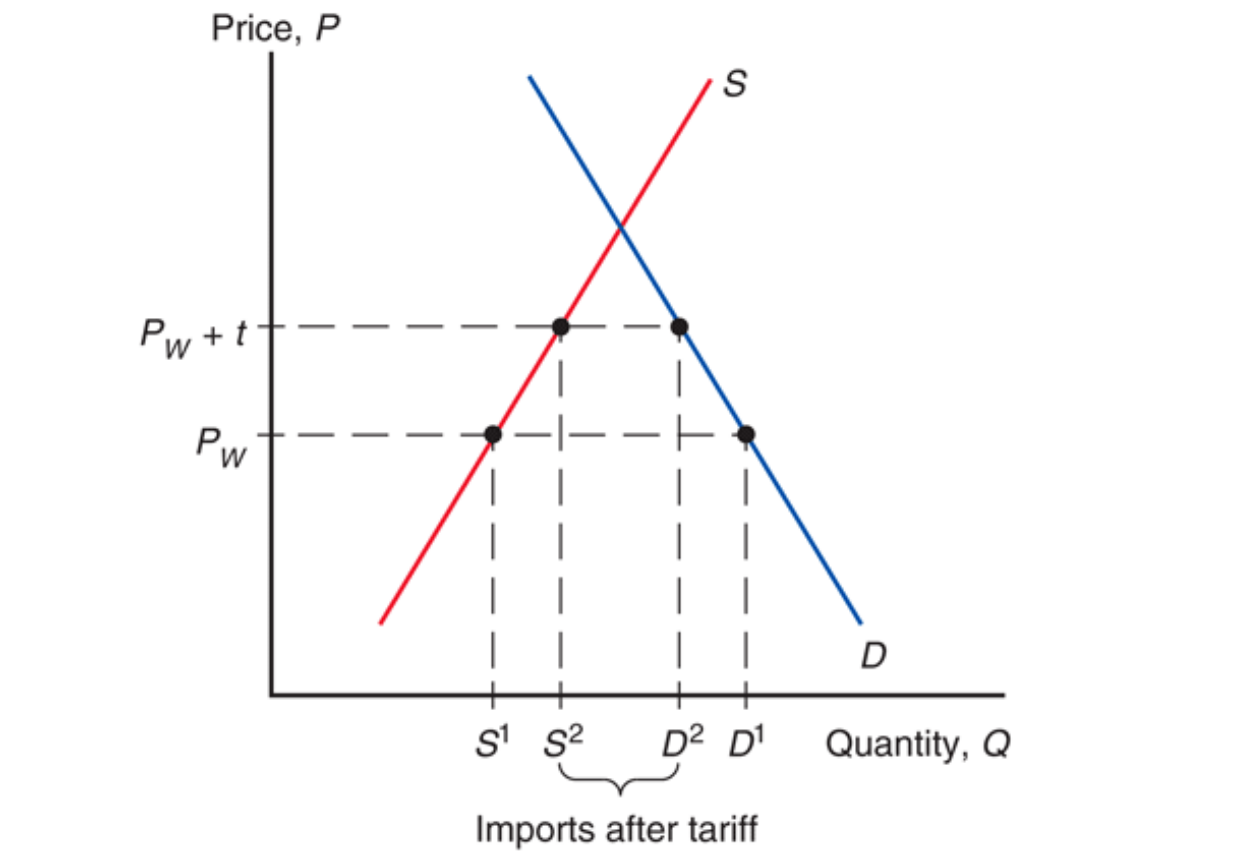
\includegraphics[width=0.80\textwidth]{flat_export_supply.png}
\end{figure}
}


\frame{
\frametitle{Evaluating the Costs and Benefits of Tariffs}
\begin{itemize}
\item A tariff raises the price of a good at Home 
\item This hurts Home consumers and helps Home producers
\item Home government also gets revenue
\end{itemize}
}

\frame{
\frametitle{Classic partial equilibrium welfare calculations}
\begin{itemize}
    \item Consumer Surplus
    \begin{itemize}
        \item Difference in the price consumer pays and the max price he is willing to pay
    \end{itemize}
    \item Producer Surplus
    \begin{itemize}
        \item Difference in at which firm sells and the min. price it would be willing to sell at
    \end{itemize}
    \item Why partial equilibrium?
    \begin{itemize}
        \item Where does producer surplus go?
        \item Workers and owners of capital are consumers
        \item The larger the producer surplus, the higher willingness to pay, etc.
        \item How does price affect prices of other goods, wages, etc?
    \end{itemize}
\end{itemize}
}

\frame{
\frametitle{Consumer Surplus}
\begin{figure}
	\centering
		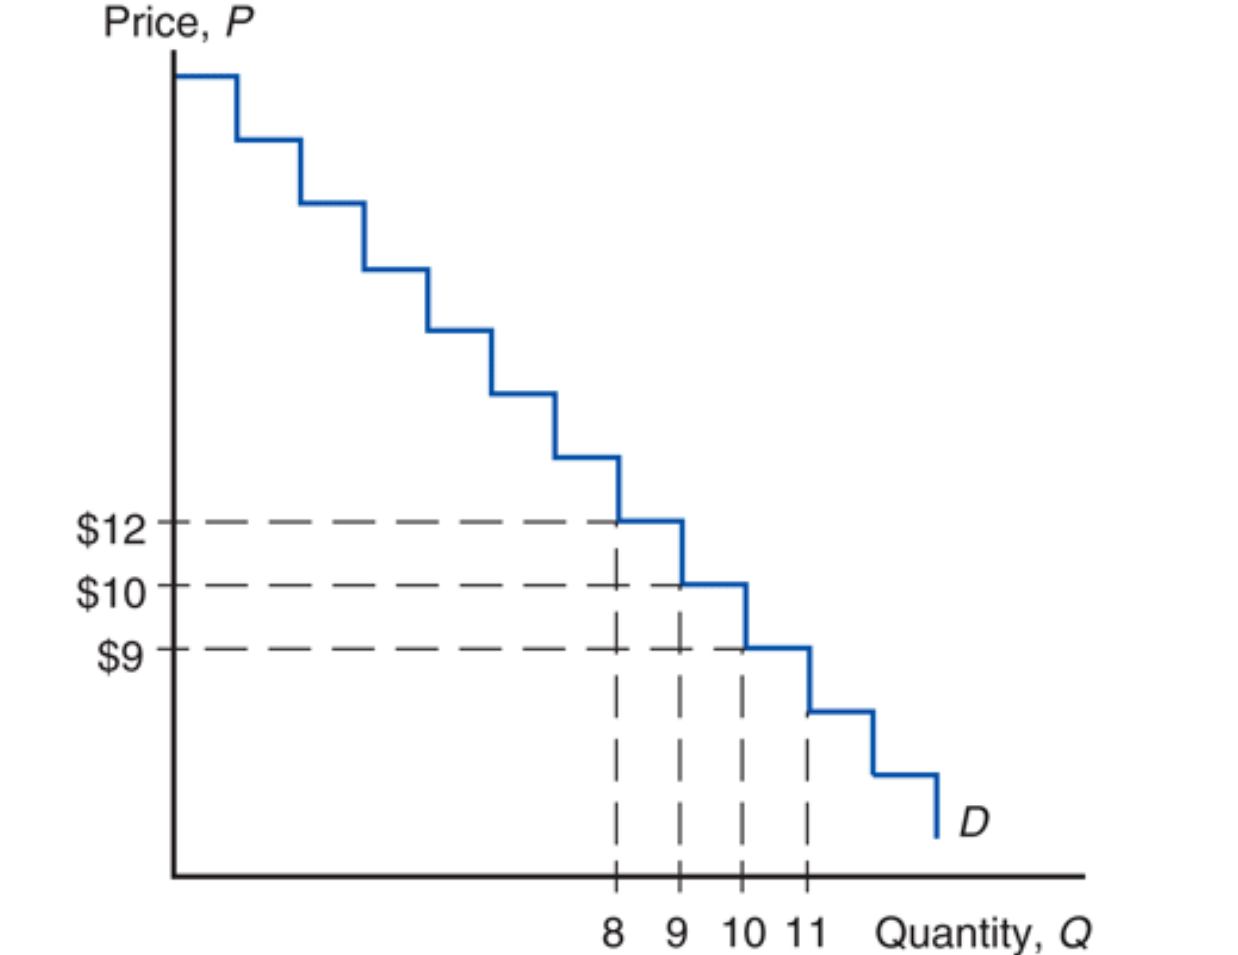
\includegraphics[width=0.80\textwidth]{demand_surplus.png}
\end{figure}
}

\frame{
\frametitle{Consumer Surplus}
\begin{figure}
	\centering
		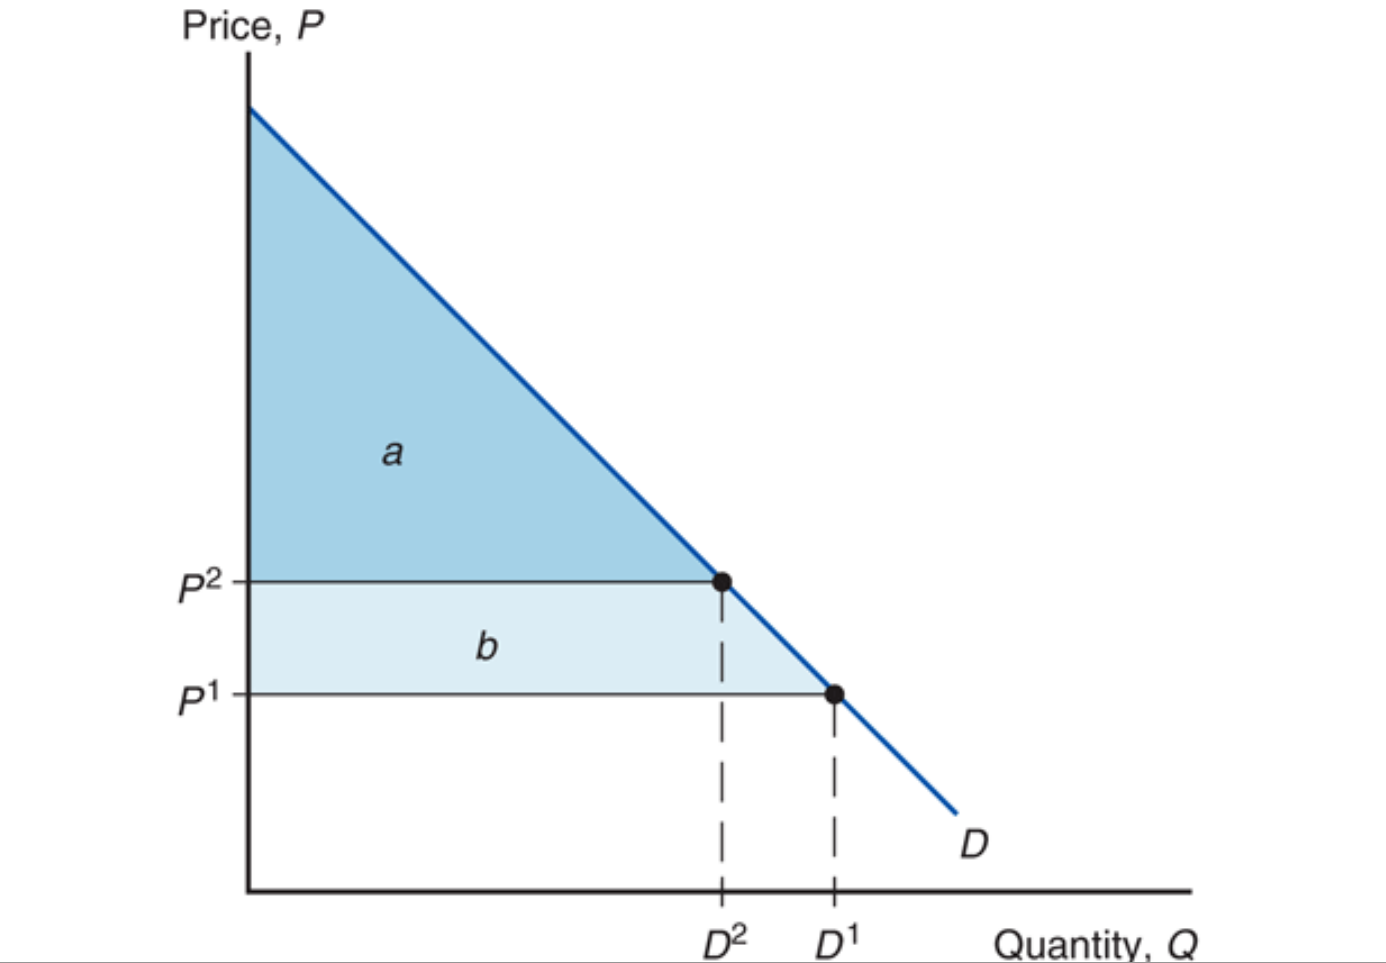
\includegraphics[width=0.80\textwidth]{consumer_surplus.png}
\end{figure}
}

\frame{
\frametitle{Producer Surplus}
\begin{figure}
	\centering
		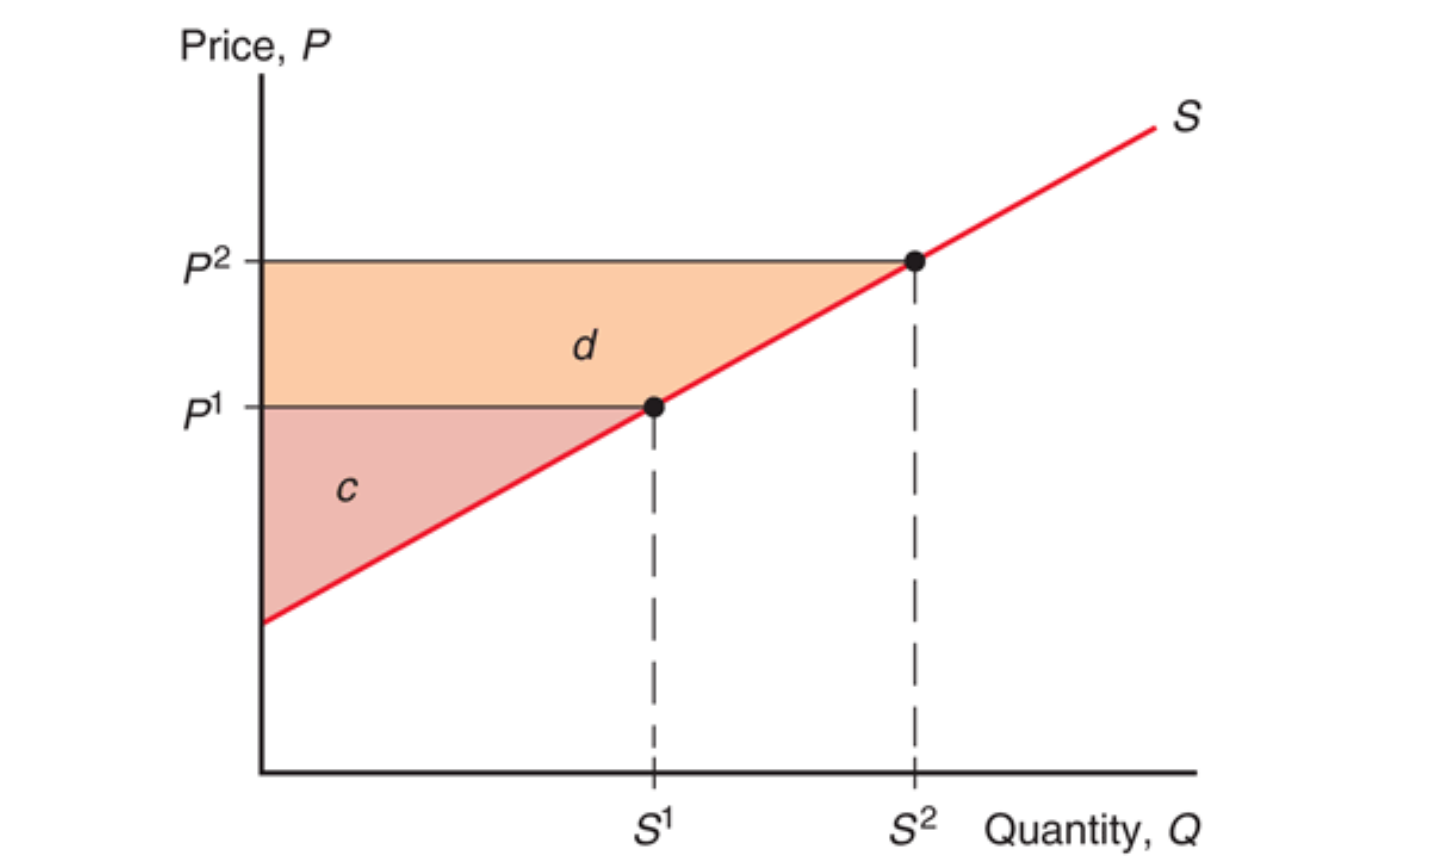
\includegraphics[width=0.80\textwidth]{producer_surplus.png}
\end{figure}
}

\begin{frame}{Effect of tariff}

    \begin{itemize}
        \item Now the effect of tariffs on consumer, producer, and government surplus
        \item Now the effect of tariffs on consumer, producer, and government surplus
        \item First Government:
        \begin{itemize}
            \item The government gets $t * Q$ in revenue
        \end{itemize}
    \end{itemize}

\end{frame}

\frame{
\frametitle{Costs and Benefits of a Tariff for the Importing Country}
\begin{figure}
	\centering
		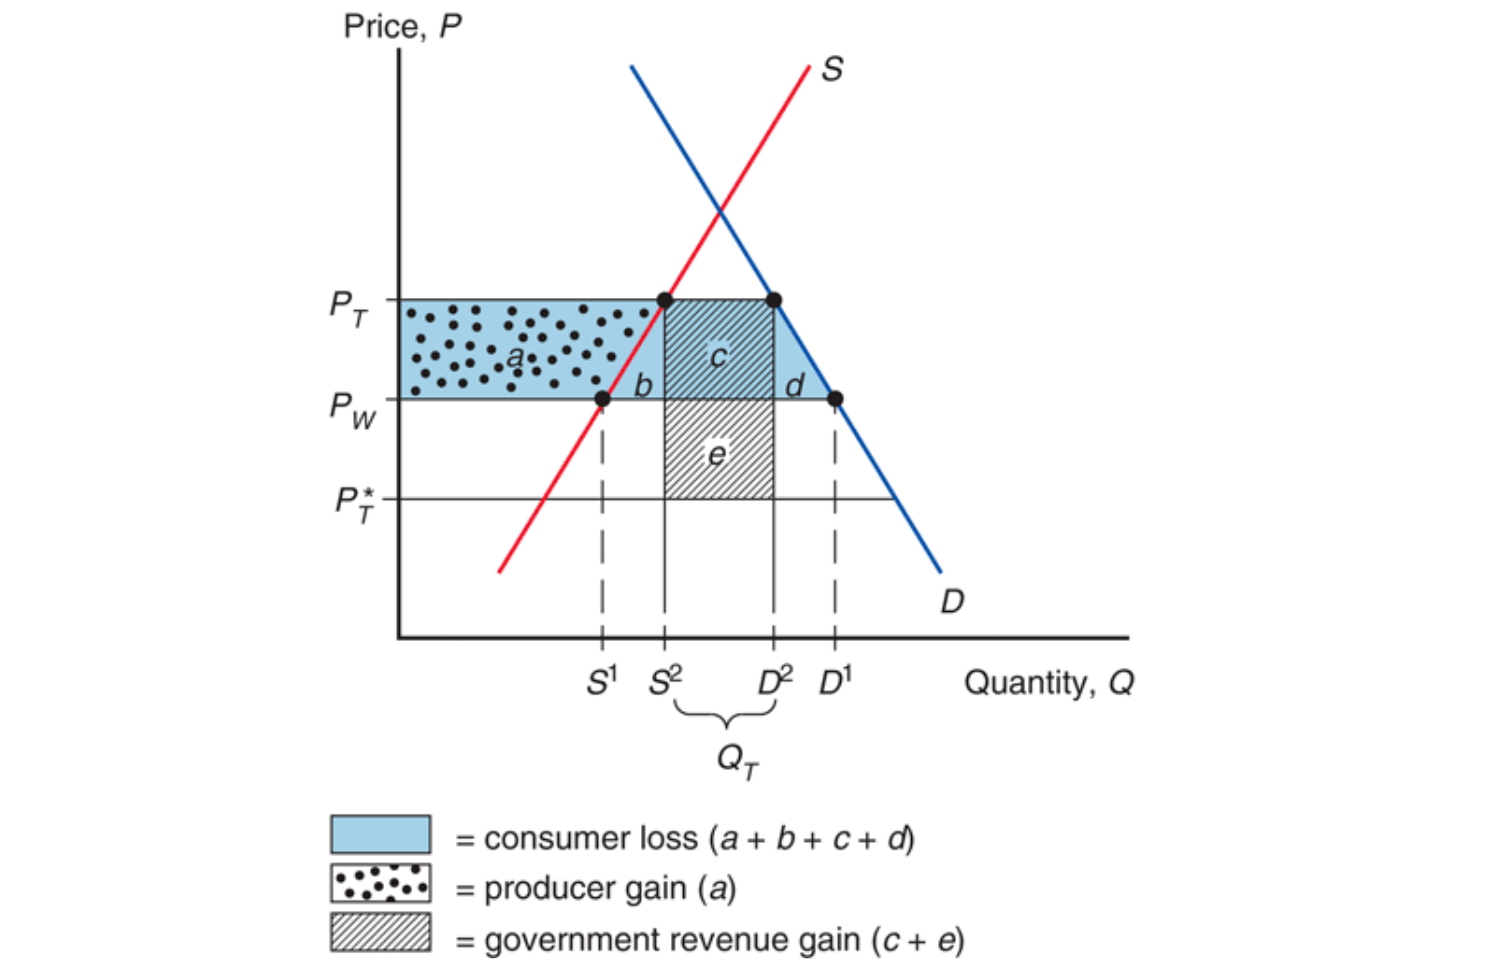
\includegraphics[scale=0.22]{tariff_effect.png}
\end{figure}
}

\begin{frame}{Effect of tariff}

    \begin{itemize}
        \item Consumers
        \begin{itemize}
            \item Lose consumer surplus between trade price and tariff price
        \end{itemize}
        \item Producers
        \begin{itemize}
            \item Gain producer surplus between trade price and tariff price
        \end{itemize}
    \end{itemize}

\end{frame}

\frame{
\frametitle{Costs and Benefits of a Tariff for the Importing Country}
\begin{figure}
	\centering
		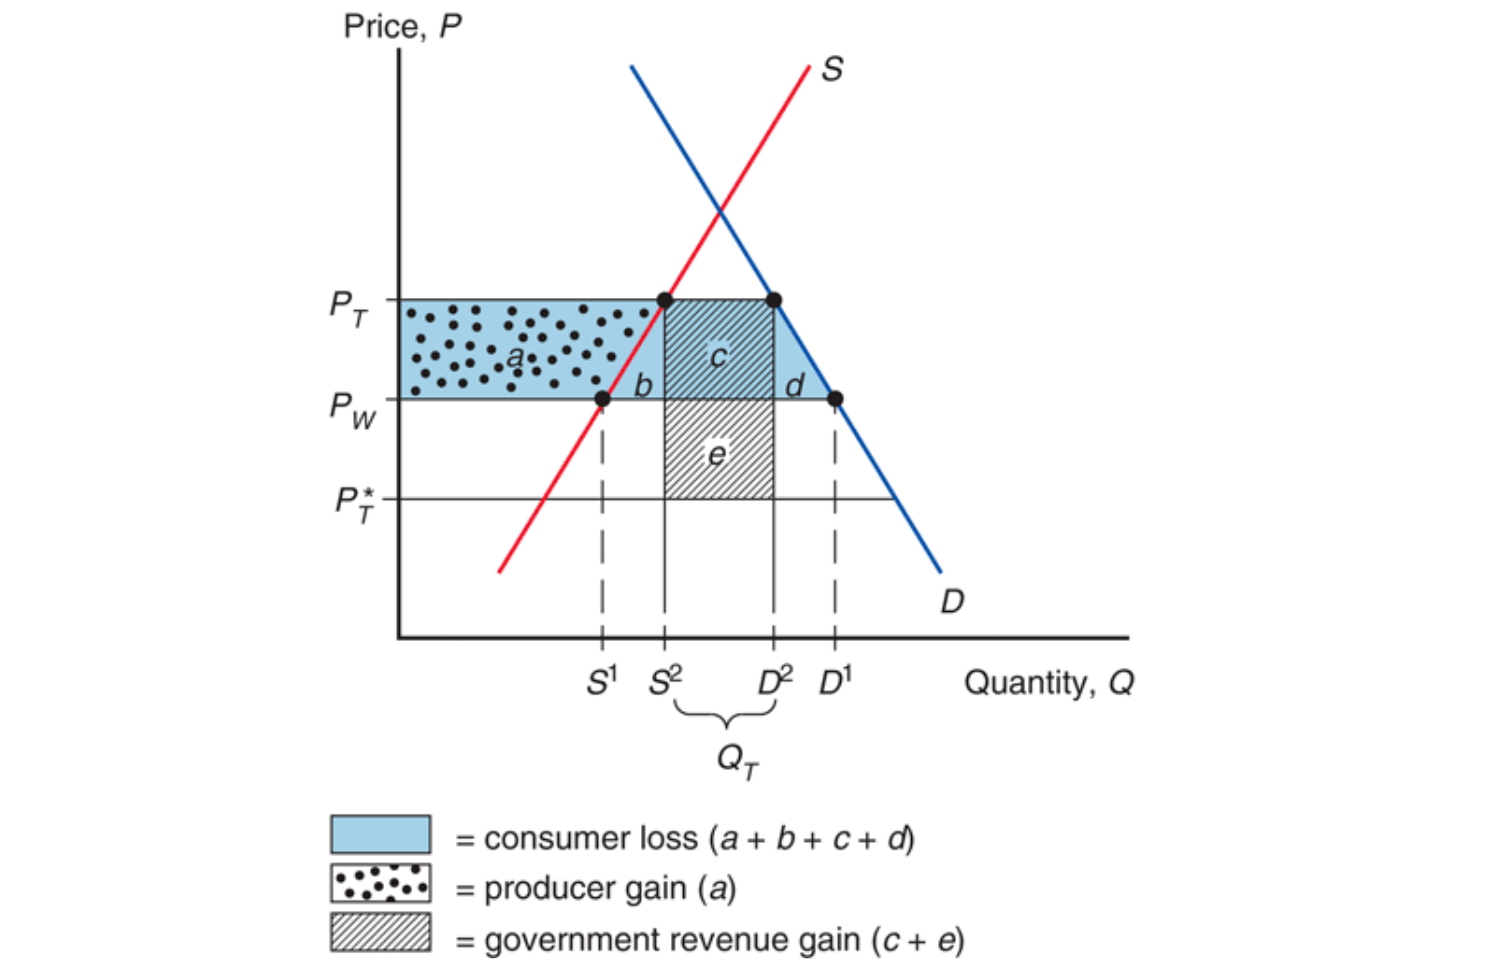
\includegraphics[scale=0.22]{tariff_effect.png}
\end{figure}
}

\frame{
\frametitle{Net gains vs losses}
\begin{figure}
	\centering
		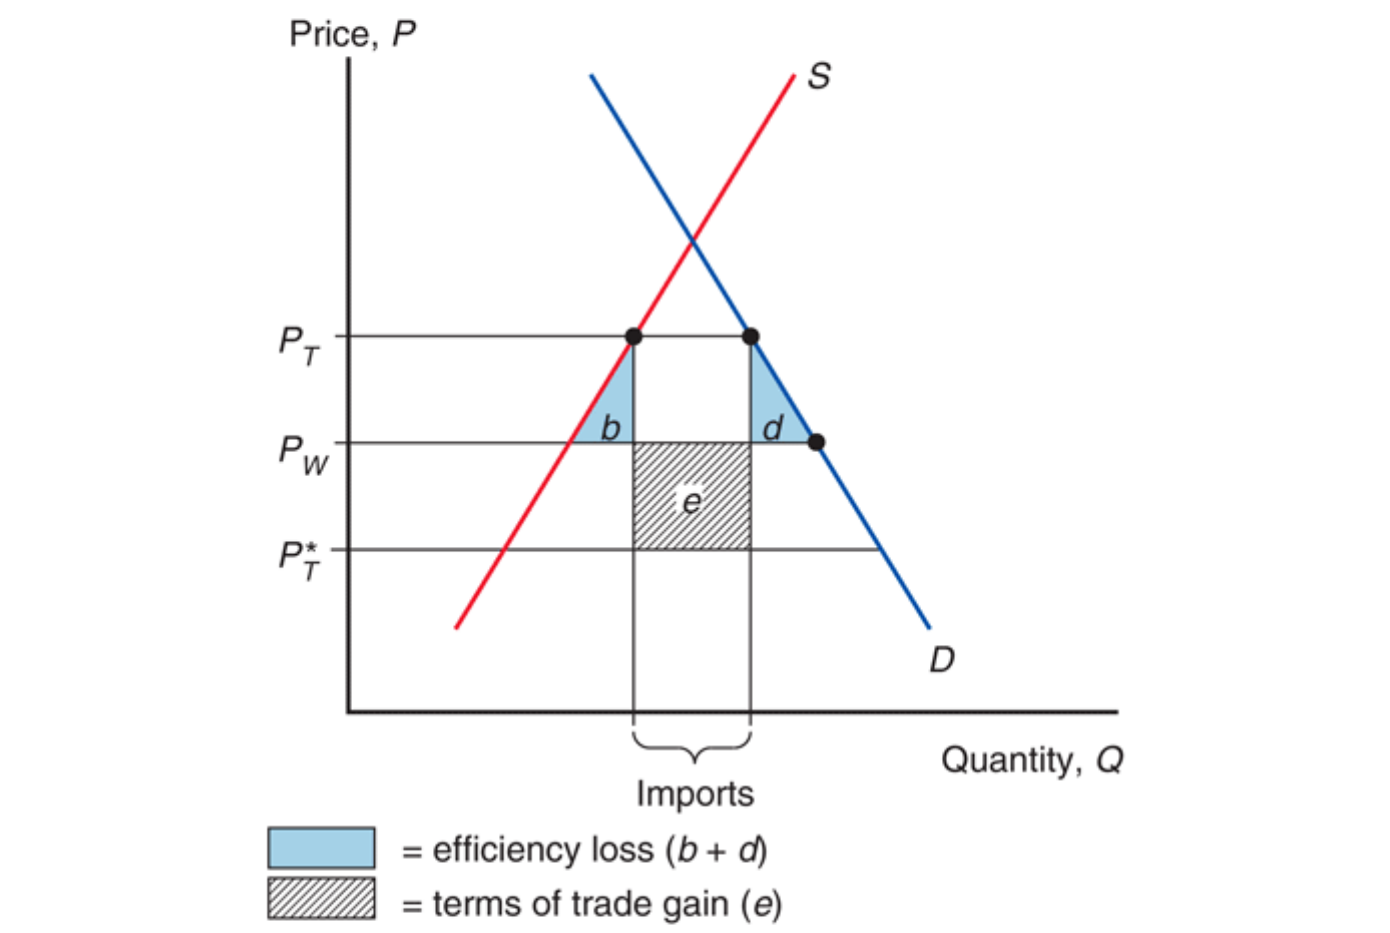
\includegraphics[scale=0.22]{net_gains.png}
\end{figure}
}

\begin{frame}{Effect of tariff}

    \begin{itemize}
        \item Punchline
        \begin{itemize}
            \item Gains from government revenue
            \item Losses from consumer surplus
        \end{itemize}
        \item What happens if Home is small?
    \end{itemize}

\end{frame}

\begin{frame}{Pause}

    \begin{itemize}
        \item We have seen that tariffs have costs and benefits
        \item Now we will analyze some other trade policy tools
        \begin{enumerate}
            \item Export subsidies (agricultural policy)
            \item Import quotas
            \item Voluntary export restraint
        \end{enumerate}
        \item Preview: All worse than tariff
        \item Reason: Others get tariff government rents
    \end{itemize}

\end{frame}

\frame{
\frametitle{Export Subsidy}
\begin{itemize}
    \item Suppose every time a firm exports a good, Foreign pays it $t$
    \item Raises the price at Foreign, while lowering it in Home
    \item Exactly the opposite of a tariff 
\end{itemize}
}

\frame{
\frametitle{Tariff and Price}
    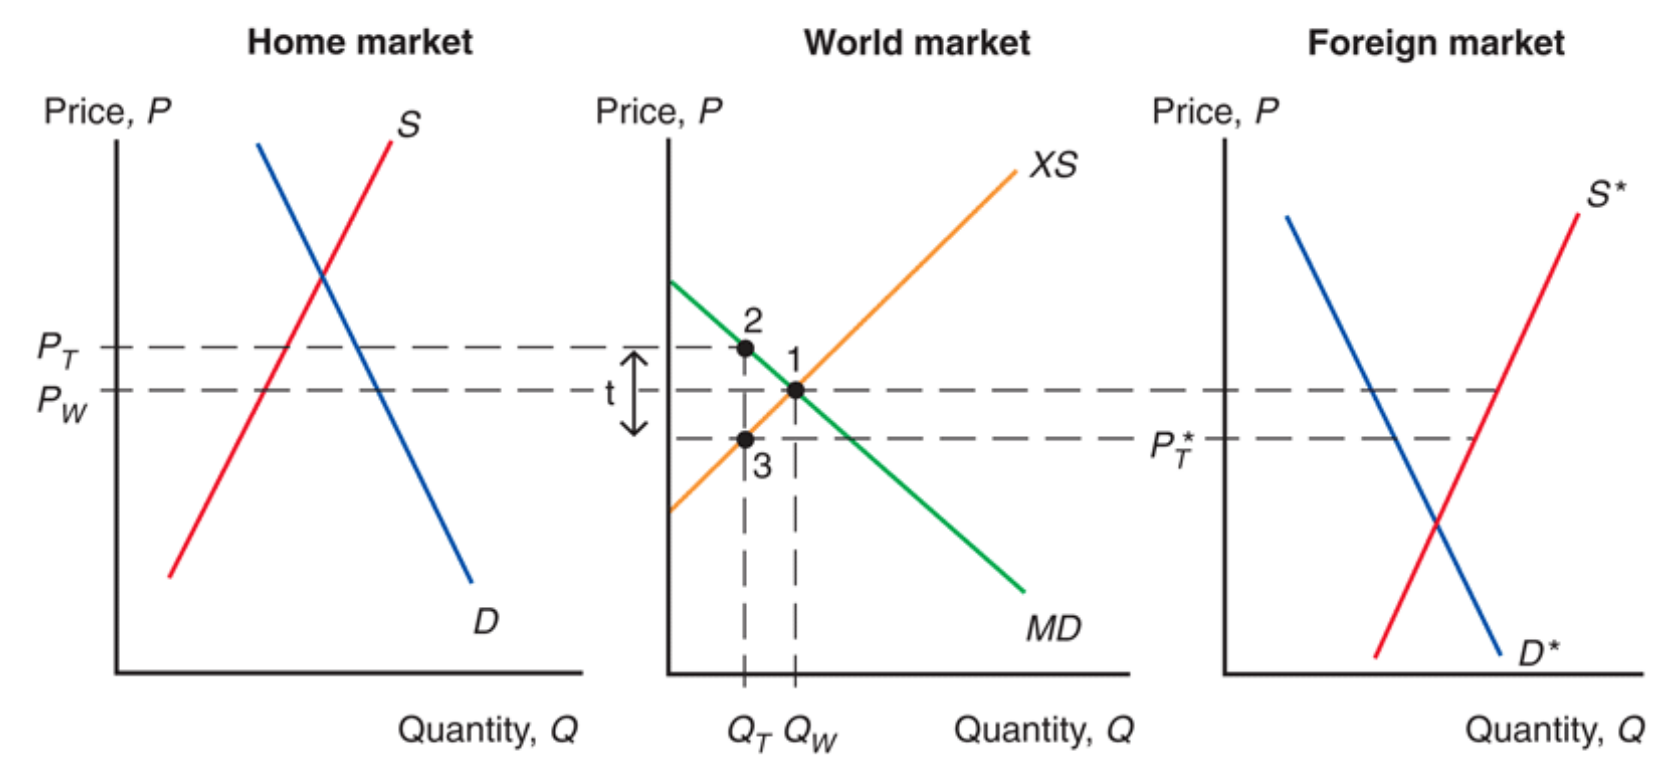
\includegraphics[width=0.80\textwidth]{tariff_prices.png}
}

\frame{
\frametitle{Gains and Losses From Export Subsidy}
\begin{itemize}
    \item Government in Foreign
    \begin{itemize}
        \item Loses $t Q$
    \end{itemize}
    \item Consumers in Foreign
    \begin{itemize}
        \item Lose are consumer surplus between world price and domestic price
    \end{itemize}
    \item Producers in Foreign
    \begin{itemize}
        \item gain producer surplus between world price and domestic price
    \end{itemize}
\end{itemize}
}


\frame{
\frametitle{Effects of an Export Subsidy}
\begin{figure}
	\centering
		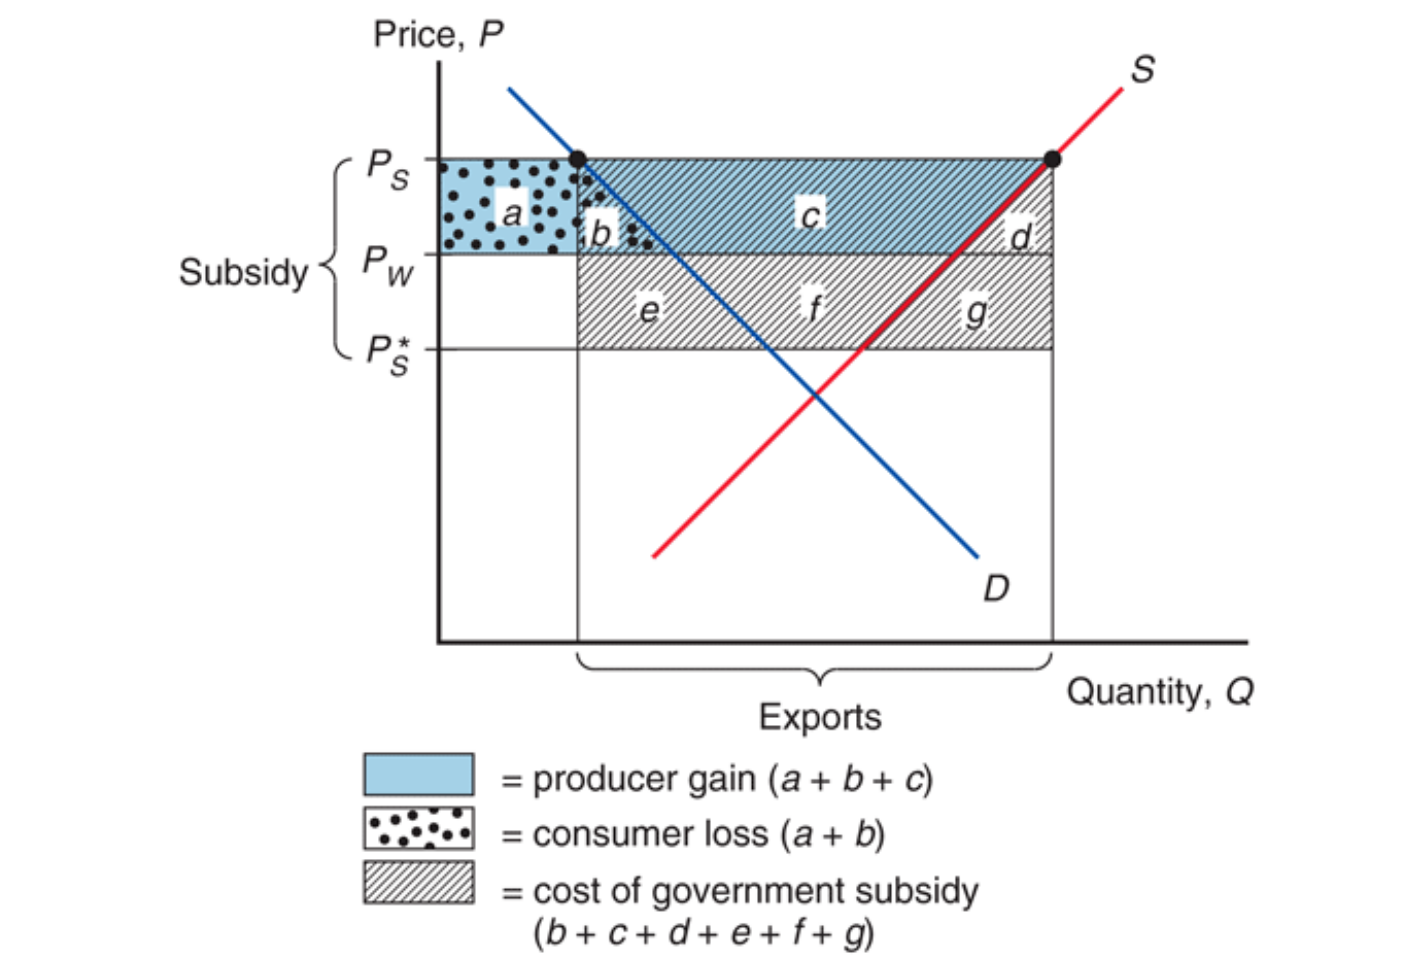
\includegraphics[scale=0.25]{export_subsidy.png}
\end{figure}
}

\frame{
\frametitle{The incredible European Agricultural Subsidy}
\begin{itemize}
    \item Flips Europe into exporting agriculture
    \item 21.5 billion Euro annual loss (exceeding gains to producers!)
\end{itemize}
		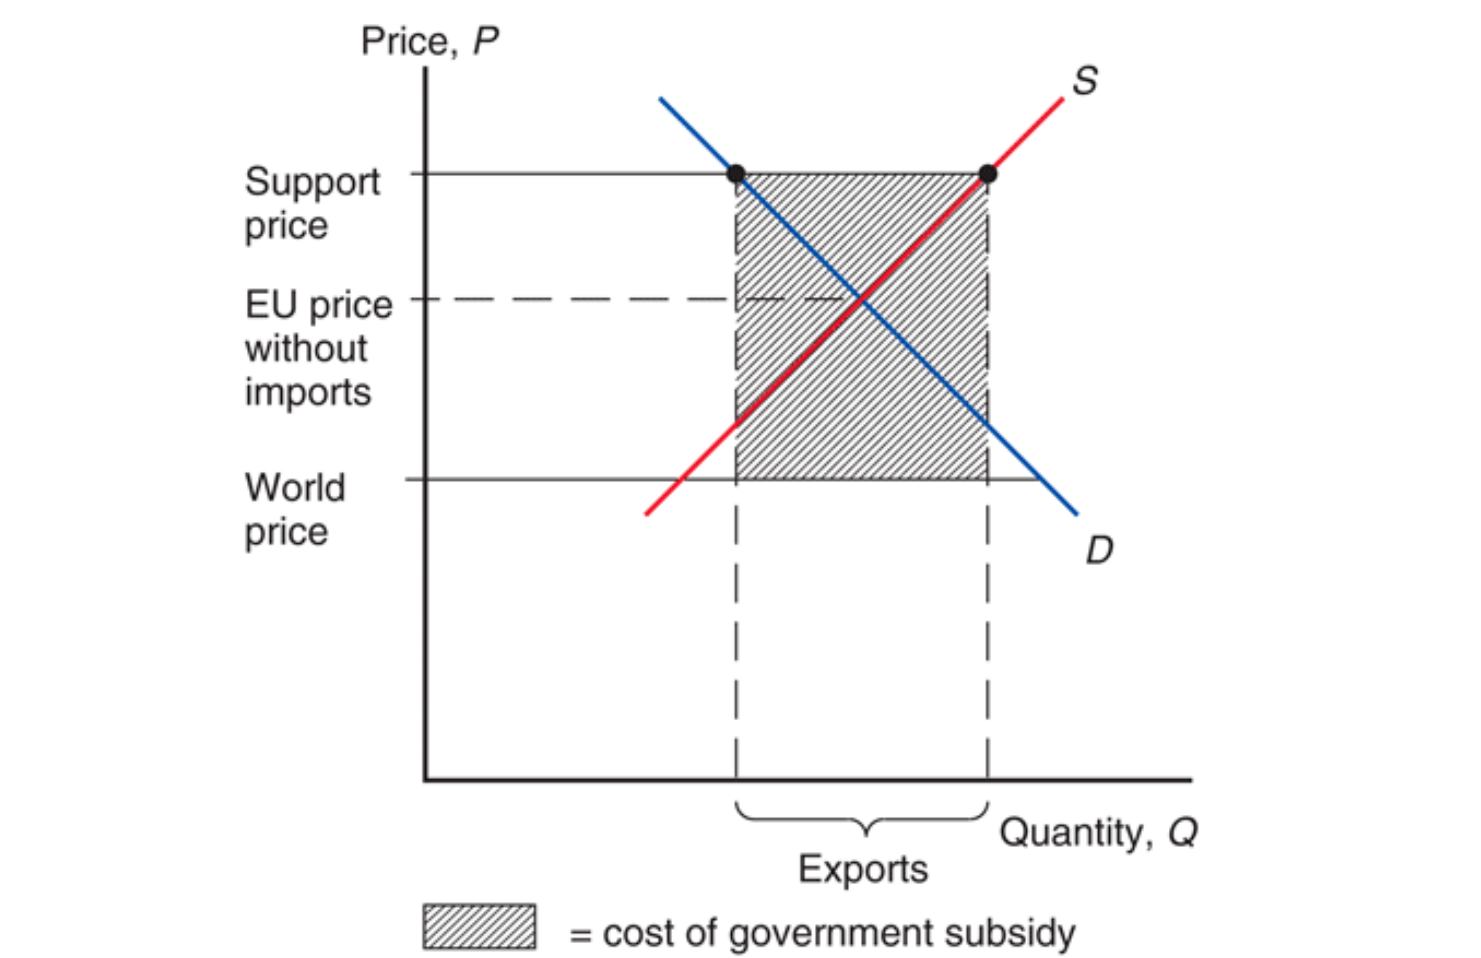
\includegraphics[scale=0.20]{export_subsidy_europe.png}
}

\frame{
\frametitle{Import Quota}
\begin{itemize}
\item Restriction on the quantity of a good that may be imported.
\item Import quota raises price of imported good, just like a tariff
\item Main difference: government doesn't get revenue!
\item Whoever gets the import licenses gets revenue
\end{itemize}
}

\frame{
\frametitle{US Sugar quota}
		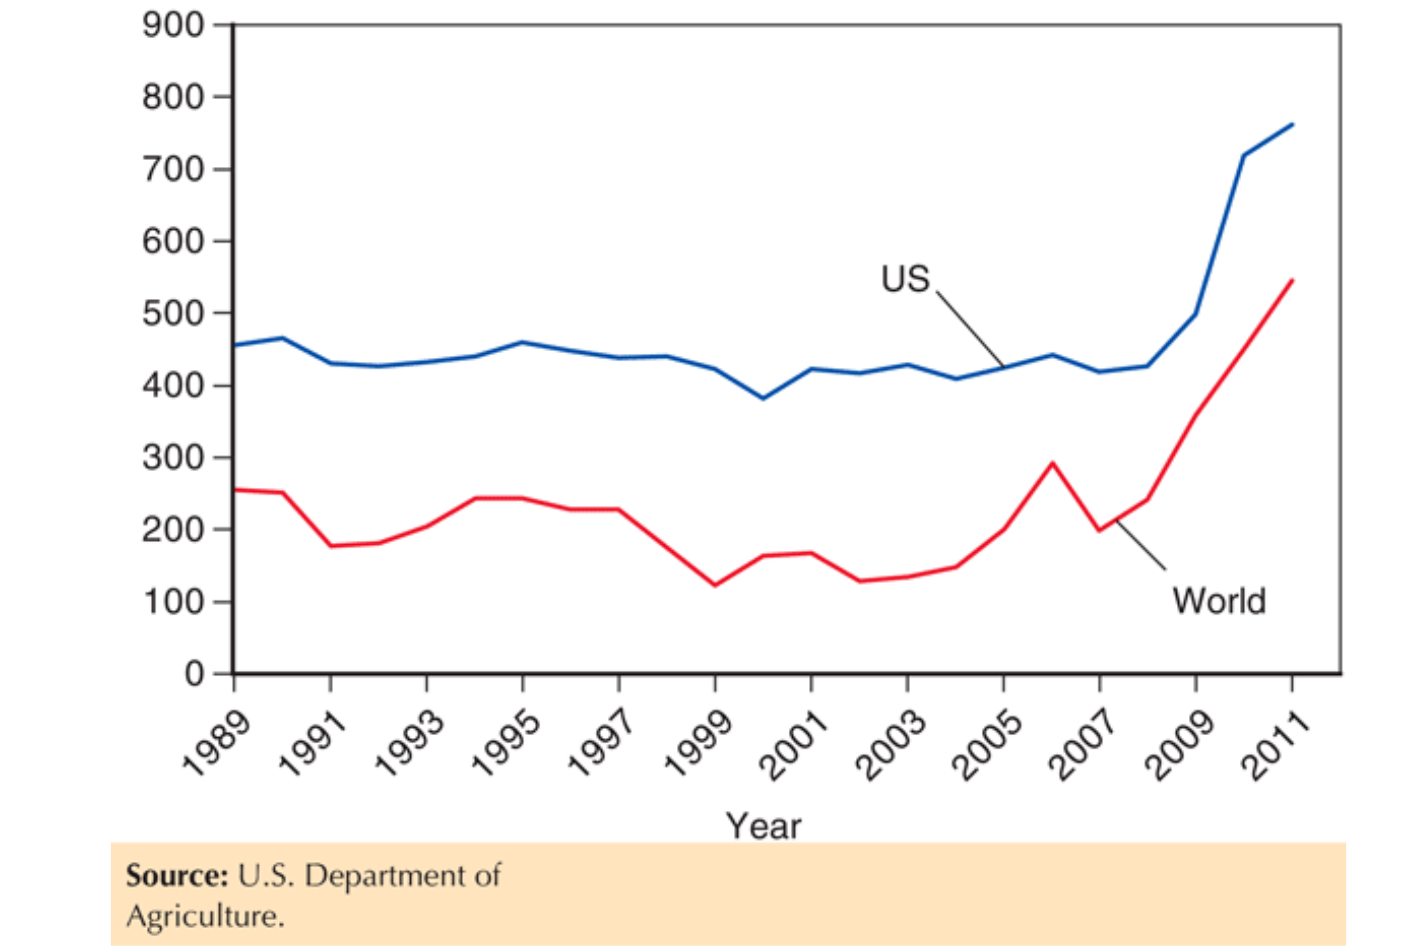
\includegraphics[scale=0.20]{us_sugar.png}
}

\frame{
\frametitle{US Sugar quota}
\begin{itemize}
    \item textbook: \emph{If the sugar restrictions were lifted, the drop in the refined sugar price would induce a substantial expansion in the sugar-using food industry}
    \item Maybe we should keep the quota\dots
\end{itemize}
    \begin{center}
		
\includegraphics[scale=0.25]{fat-american.jpg}
    \end{center}
}

\frame{
\frametitle{Voluntary Export Restraint}
\begin{itemize}
\item Typically imposed by exporter at request of importer under threat of tariffs
\item Just like an import quota except\dots
\item The rents go to whoever exporter wants
\end{itemize}
}

\frame{
\frametitle{Voluntary Export Restraint}
\begin{itemize}
\item Typically imposed by exporter at request of importer under threat of tariffs
\item Just like an import quota except\dots
\item The rents go to whoever exporter wants
\end{itemize}
}

\frame{
\frametitle{Summary}
\begin{figure}
	\centering
		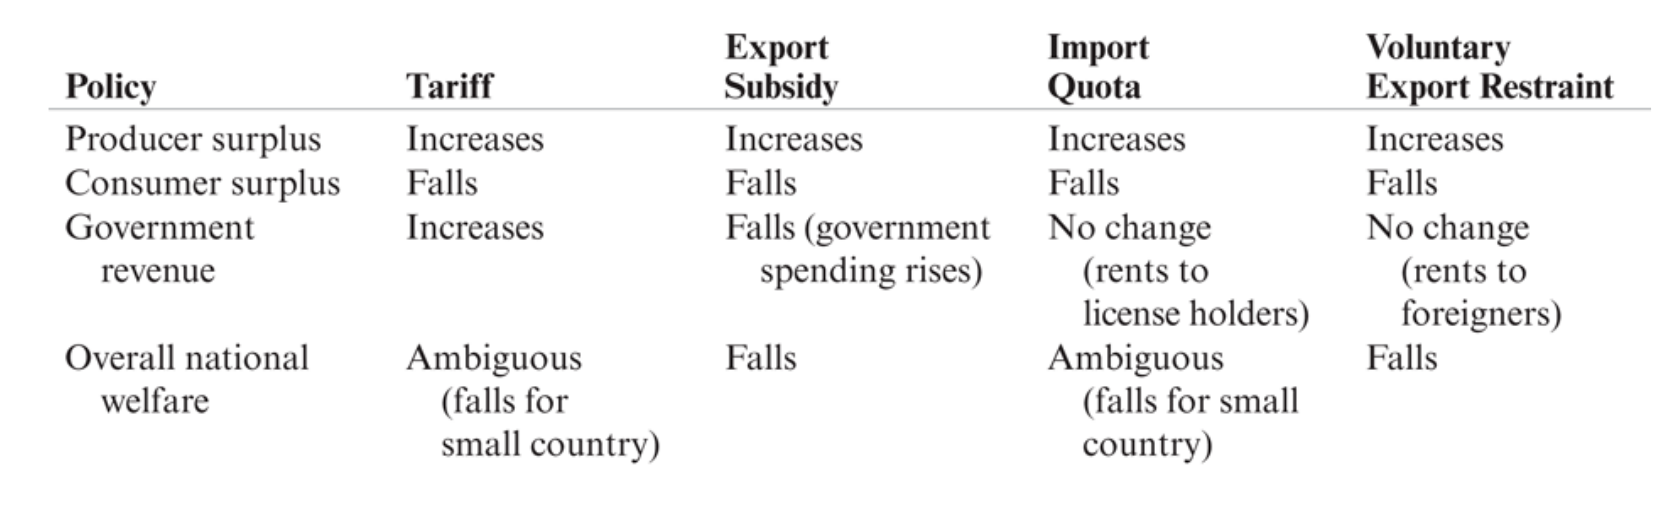
\includegraphics[scale=0.20]{summary_table.png}
\end{figure}}

\begin{frame}{Summary}
    \begin{itemize}
        \item Partial equilibrium analysis of tariffs
        \begin{itemize}
            \item Can be good, can be bad
        \end{itemize}
        \item Everything else bad
        \begin{itemize}
            \item Export subsidies crazy bad
        \end{itemize}
        \item So why do governments have all sorts of trade policy?
        \begin{itemize}
            \item Political considerations, Chapter 10
            \item Next time, Chp. 10, 11, and 12
        \end{itemize}
    \end{itemize}
\end{frame}

\begin{frame}{Bonus!}
    \begin{itemize}
        \item Proof that always an optimal tariff (appendix to chp. 10)
    \end{itemize}
\end{frame}

\end{document}

